\documentclass[12pt]{article}
\usepackage[utf8]{inputenc}
\usepackage[russian]{babel}
\usepackage{graphicx}
\usepackage{listings}
\usepackage{indentfirst}
\usepackage{color}
\usepackage{multirow}
\usepackage{amsmath}
\usepackage{bm}
\usepackage{tikz}

\definecolor{dkgreen}{rgb}{0,0.6,0}
\definecolor{gray}{rgb}{0.5,0.5,0.5}
\definecolor{ltgray}{rgb}{0.95,0.95,0.95}
\definecolor{mauve}{rgb}{0.58,0,0.82}
\newcommand{\rot}{\mathop{\rm rot}\nolimits}
\renewcommand{\lstlistingname}{Листинг}
\lstset{ %
  language=Python,                % the language of the code
  basicstyle=\footnotesize\ttfamily,           % the size of the fonts that are used for the code
%  numbers=left,                   % where to put the line-numbers
%  numberstyle=\tiny\color{gray},  % the style that is used for the line-numbers
%  stepnumber=2,                   % the step between two line-numbers. If it's 1, each line 
                                  % will be numbered
%  numbersep=5pt,                  % how far the line-numbers are from the code
  backgroundcolor=\color{ltgray},      % choose the background color. You must add \usepackage{color}
  showspaces=false,               % show spaces adding particular underscores
  showstringspaces=false,         % underline spaces within strings
  showtabs=false,                 % show tabs within strings adding particular underscores
  %frame=single,                   % adds a frame around the code
  rulecolor=\color{black},        % if not set, the frame-color may be changed on line-breaks within not-black text (e.g. comments (green here))
  columns=fixed,
  tabsize=2,                      % sets default tabsize to 2 spaces
  captionpos=b,                   % sets the caption-position to bottom
  breaklines=true,                % sets automatic line breaking
  breakatwhitespace=false,        % sets if automatic breaks should only happen at whitespace
%  caption=Valalala,                   % show the filename of files included with \lstinputlisting;
                                  % also try caption instead of title
  keywordstyle=\color{blue},          % keyword style
  commentstyle=\color{gray},       % comment style
  stringstyle=\color{dkgreen},         % string literal style
  escapeinside={\%*}{*)},            % if you want to add LaTeX within your code
  morekeywords={*,...},              % if you want to add more keywords to the set
  deletekeywords={...}              % if you want to delete keywords from the given language
}


\title{Численное сравнение схем расщепления для нестационарного уравнения Стокса}
\author{Борисов В.С.}

\begin{document}

\maketitle

\begin{abstract}
Рассматривается применение схем расщепления для нестационарного уравнения Стокса, которое описывает течение сильно вязкой несжимаемой жидкости. 
Исходная система уравнений для давления и скорости решается численно с применением схем расщепления. 
Проведено сравнение времени, погрешности вычисления с решениями без расщепления.
\end{abstract}

\section{Математическая модель}
Нестационарное уравнение Стокса, описывает течение несжимаемой жидкости в области $\Omega$ с границей $\partial \Omega$:
\begin{equation*}
\begin{aligned}
\frac{\partial {\bm u}}{\partial t} -\Delta {\bm u} + \nabla p &= {\bm f}({\bm x}, t), \\
\nabla\cdot{\bm u} &= 0, 
\end{aligned}
\quad {\bm x} \in \Omega, \quad 0<t \leq T,
\end{equation*} 
$$
\begin{aligned}
{\bm u({\bm x}, 0)} &= {\bm u^0}({\bm x}), \quad {\bm x} \in \Omega, \\
{\bm u({\bm x}, t)} &= {\bm g}({\bm x}, t), \quad {\bm x} \in \partial\Omega, \quad 0<t \leq T,
\end{aligned}
$$
где ${\bm u}({\bm x}, t)$ - скорость, $p({\bm x}, t)$ - давление и ${\bm f}({\bm x}, t)$ - внутренний источник движения. В двумерном случае ${\bm x}=(x_1, x_2)$.

В качестве тестовой модельной задачи, возьмем задачу о течении в каверне с подвижной верхней границей. 
Для задания подвижной границы, необходимо задать на ней ненулевые значения скорости.
Задача решается на единичном квадрате $\Omega$ (рис. \ref{fg:cavity}), c границей $\partial \Omega=\Gamma_1 \cup \Gamma_2$. На верхней границе $\Gamma_1$ поставлено условие гладкой стенки $({\bm u}, {\bm n}) = 0$, где ${\bm n}$ нормаль границы и движение идет по направлению границы (направо ${\bm g}({\bm x},t)=\{1,0\}$). 
В остальной части границы $\Gamma_2=\partial \Omega / \Gamma_1$ поставлено условие прилипания ${\bm g}({\bm x}, t)={\bm 0}$. Внутренние источники скорости отсутствуют ${\bm f}({\bm x}, t)={\bm 0}$. Таким образом, решаемая задача имеет следующую постановку:
\begin{equation}
\begin{aligned}
\frac{\partial {\bm u}}{\partial t} -\Delta {\bm u} + \nabla p &= {\bm 0}, \\
\nabla\cdot{\bm u} &= 0, 
\end{aligned}
\quad {\bm x} \in \Omega, \quad 0<t \leq T,
\label{eq:scheme-main}
\end{equation} 
с граничными условиями:
\begin{equation}
\begin{split}
{\bm u({\bm x}, t)} &= \{1, 0\}, \quad {\bm x} \in \Gamma_1, \\
{\bm u({\bm x}, t)} &= {\bm 0}, \quad {\bm x} \in \Gamma_2, \\
\end{split}
\quad 0<t \leq T,
\label{eq:scheme-boundary}
\end{equation} 
и начальным условием:
\begin{equation}
{\bm u({\bm x}, 0)} = {\bm 0}, \quad {\bm x} \in \Omega.
\label{eq:scheme-start}
\end{equation}

\begin{figure}
	\begin{center}
\begin{tikzpicture}
	\tikzstyle{every node} =[font=\large];
	\path [fill=gray!20!white] (0,0) -- (0, 5) -- (5, 5) -- (5, 0) -- (0, 0);    
	\draw [<->, line width=2](6,0) -- (0, 0) -- (0, 6);    
    	\draw [blue, line width=2] (0,0) -- (0, 5) -- (5, 5) -- (5, 0) -- (0, 0);    
    \draw [red, line width=2] (0, 5) -- (5, 5);
    \node at (-0.5, -0.5) {$0$};
    \node at (-0.5, 6) {$x_2$};
    \node at (6, -0.5) {$x_1$};
    \node at (-0.5, 5) {$1$};
    \node at (5, -0.5) {$1$};
    
    \node at (2.5, 4.5) {${\bm u} = \{1, 0\}$};
    %\node at (4.5, 2.5) {${\bm u} = {\bm 0}$};
    %\node at (0.5, 2.5) {${\bm u} = {\bm 0}$};
    \node at (2.5, 0.5) {${\bm u} = {\bm 0}$};
    
    \node at (2.5, 5.5) {$\Gamma_1$};    
    \node at (2.5, -0.5) {$\Gamma_2$};
    \node at (-0.5, 2.5) {$\Gamma_2$};
    \node at (5.5, 2.5) {$\Gamma_2$};
    
    \node at (2.5, 2.5) {$\Omega$};
\end{tikzpicture}
		\caption{Расчетная область.}
		\label{fg:cavity}
	\end{center}
\end{figure}

\section{Вариационная постановка}
Для численного решения задачи методом конечных элементов, уравнение (\ref{eq:scheme-main}) необходимо привести к вариационной постановке \cite{fenicsbook-2012}. Введем следующие функциональные пространства \cite{guzman-2011}:
$$
V=\{ ({\bm u}, p) : \, {\bm u} \in H(\mathrm{div}, \Omega), \, p \in L^2(\Omega),  {\bm u}|_{\partial \Omega}= {\bm g} \},
$$
$$
\hat V=\{ ({\bm v}, q) : \, {\bm v} \in H(\mathrm{div}, \Omega), \, q \in L^2(\Omega), \, {\bm v}|_{\partial \Omega}={\bm 0} \},
$$
где $L^2(\Omega)$ --- гильбертово пространство, $H(\mathrm{div}, \Omega) = \{{\bm u} \in [L^2(\Omega)]^2 : \nabla\cdot {\bm u} \in L^2(\Omega)\}$ --- функциональное пространство Соболева.
Умножим уравнения (\ref{eq:scheme-main}) с неизвестными функциями $({\bm u}, p) \in V$  на тестовые функции $({\bm v}, q)$ соответственно, и возьмем интеграл по области $\Omega$:
$$
\begin{aligned}
\int_{\Omega} \frac{\partial {\bm u}}{\partial t} \cdot {\bm v} \,dx - \int_{\Omega} \Delta {\bm u} \cdot {\bm v} \,dx + \int_{\Omega} \nabla p \cdot {\bm v} \,dx = 0, \\
\int_{\Omega} (\nabla \cdot {\bm u}) \cdot q \,dx = 0.
\end{aligned}
\quad \forall ({\bm v},q) \in \hat V,
$$
Используя формулу Грина, преобразуем уравнение:
$$
\int_{\Omega} \frac{\partial {\bm u}}{\partial t} \cdot {\bm v} \,dx + \int_{\Omega} \nabla {\bm u} \cdot \nabla {\bm v} \,dx - \int_{\partial \Omega} \frac{\partial {\bm u}}{\partial {\bm n}} \cdot {\bm v} \,dS + \int_{\Omega} \nabla p \cdot {\bm v} \,dx = 0,
$$
здесь интеграл по $\partial \Omega$ равен нулю, т.к. функция ${\bm v} | _ {\partial \Omega} = 0$. Поэтому:
$$
\int_{\Omega} \frac{\partial {\bm u}}{\partial t} \cdot {\bm v} \,dx + \int_{\Omega} \nabla {\bm u} \cdot \nabla {\bm v} \,dx - \int_{\Omega} \nabla p \cdot {\bm v} \,dx = 0.
$$
Вариационная постановка --- найти $({\bm u}, p) \in V$ такие что:
$$
\int_{\Omega} \frac{\partial {\bm u}}{\partial t} \cdot {\bm v} \,dx + \int_{\Omega} \nabla {\bm u} \cdot \nabla {\bm v} \,dx + \int_{\Omega} \nabla p \cdot {\bm v} \,dx = 0, 
$$
$$
\int_{\Omega} (\nabla \cdot {\bm u}) \cdot q \,dx = 0, \quad ({\bm v}, q) \in \hat V,
$$
с граничными и начальным условиями (\ref{eq:scheme-boundary}) и (\ref{eq:scheme-start}) соответственно.

\section{Схемы без расщепления}
Здесь рассмотрены две схемы, которые являются частными случаями схемы с весами.
Скорость и давление вычисляются как единая переменная в системе уравнений. 
Для поиска решения методом конечных элементов, введем подпространства сеточных функций $V_h \subset V$ и  ${\hat V}_h \subset {\hat V}$.
Введем равномерную сетку по времени $\omega_t=\{t^n=n\tau, \, n=0,1,...,N, \, \tau N = T \}$, и определим ${\bm u}_h^n={\bm u}({\bm x}, t^n)$ где $t^n=n\tau$. Решение системы вычисляется как общая сеточная функция $({\bm u}_h^{n+1}, p_h^{n+1}) \in V_h$. После ее определения, функции для скорости и давления находятся путем разделения.

\subsection{Чисто неявная схема} 
Чисто неявная схема приведена для сравнения точности со схемами расщепления. 
Погрешность аппроксимации по времени $O(\tau)$.
Найти такие $({\bm u}_h^{n+1}, p_h^{n+1}) \in V_h$ для задачи:
\begin{equation} \label{eq:scheme-impl-1}
\frac{1}{\tau} \int_\Omega {\bm u_h^{n+1}} \cdot {\bm v} \, dx + \int_\Omega \nabla {\bm u_h^{n+1}} \cdot \nabla {\bm v} \, dx + \int_\Omega {\bm v} \cdot \nabla p_h^{n+1} \, dx = \frac{1}{\tau} \int_\Omega {\bm u}_h^n \cdot {\bm v} \, dx, 
\end{equation}
$$
\int_\Omega q \nabla \cdot {\bm u_h^{n+1}} \, dx = 0, \quad \forall ({\bm v},q) \in \hat V_h.
$$

\subsection{Схема Кранка-Николсона} 
Схема приведена для сравнения точности со схемами расщепления.
Погрешность аппроксимации по времени $O(\tau^2)$.
Найти такие $({\bm u}_h^{n+1}, p_h^{n+1}) \in V_h$ для задачи:
\begin{eqnarray*}
\frac{1}{\tau} \int_\Omega {\bm u_h^{n+1}} \cdot {\bm v} \, dx + \frac{1}{2} \int_\Omega \nabla {\bm u_h^{n+1}} \cdot \nabla {\bm v} \, dx + \int_\Omega {\bm v} \cdot \nabla p_h^{n+1} \, dx = \nonumber\\  = \frac{1}{\tau} \int_\Omega {\bm u}_h^n \cdot {\bm v} \, dx - \frac{1}{2} \int_\Omega \nabla {\bm u}_h^n \cdot \nabla {\bm v} \, dx - \int_\Omega {\bm v} \cdot \nabla p_h^{n} \, dx ,
\end{eqnarray*}
$$
\int_\Omega q \nabla \cdot {\bm u_h^{n+1}} \, dx = 0, \quad \forall ({\bm v},q) \in \hat V_h.
$$

\section{Схемы расщепления}
Особенность расщепления состоит в уменьшении размера матрицы для конечной СЛАУ. Вместо составления единого смешанного пространства переменных скорости и давления, вычисления проводятся по отдельности для сеточных функций скорости и давления. При решении СЛАУ меньшего размера, происходит экономия вычислительного времени, машинной памяти и изменяется погрешность.

Показана неотрицательная определенность расщепляемых операторов.
Для каждой схемы строится отдельная вариационная постановка с использованием уже введенных пространств, принцип преобразования оператора Лапласа и избавление от интеграла по границе сохраняется. Введем ${\bm u}_h^{n+\frac{1}{2}}$ как промежуточное значение между значения скорости на различных временных слоях ${\bm u}_h^n$ и ${\bm u}_h^{n+1}$.

Введем следующие функциональные пространства \cite{guzman-2011}:
$$
H=\{ {\bm u} \in H(\mathrm{div}, \Omega), \, {\bm u}|_{\partial \Omega}= {\bm g} \},
$$
$$
\hat{H}=\{ {\bm v} \in H(\mathrm{div}, \Omega), \, {\bm v}|_{\partial \Omega}={\bm 0} \},
$$
$$
\Pi=\{ p \in L^2(\Omega) \},
$$
где $L^2(\Omega)$ --- гильбертово пространство, $H(\mathrm{div}, \Omega) = \{{\bm u} \in [L^2(\Omega)]^2 : \nabla\cdot {\bm u} \in L^2(\Omega)\}$ --- функциональное пространство Соболева. Выделим подпространства сеточных функций $H_h \subset H, \, \hat{H}_h \subset \hat{H}, \, \Pi_h \subset \Pi$.

\subsection{Расщепляемые операторы}
Уравнение (\ref{eq:scheme-main}) запишем в операторном виде:
$$
\frac{\partial {\bm u}}{\partial t} + A {\bm u} = {\bm 0},
$$
где оператор $A=A_1 + A_2$ аддитивный оператор:
$$A_1 {\bm u} = - \Delta {\bm u}, \quad {\bm u} = {\bm 0}, \quad {\bm x} \in {\partial \Omega}$$
$$A_2 {\bm u} = \nabla p, \quad \nabla \cdot {\bm u} = 0.$$
Оператор $A_1$ определен на функциях ${\bm u}$ принимающих на границе $\partial \Omega$ значение ноль вектор, $A_2$ определен при условии $\nabla \cdot {\bm u} = 0.$

Рассмотрим $(A_1 {\bm u}, {\bm u})$:
$$
\int_{\Omega} -\Delta {\bm u} \cdot {\bm u} \, dx = \int_{\Omega} (\nabla {\bm u})^2 \, dx - \int_{\partial \Omega} {\bm u} \frac{\partial {\bm u}}{\partial {\bm n}} \, dx,
$$
где интеграл по границе принимает значение ноль, по определению оператора $A_1$. Таким образом $(A_1 {\bm u}, {\bm u}) \geq 0$.

Рассмотрим  $(A_2 {\bm u}, {\bm u})$, используем свойство дивергенции для раскрытия интеграла:
$$
\int_{\Omega} \nabla p \cdot {\bm u} \, dx = \int_{\Omega} \nabla \cdot (p{\bm u}) \, dx - \int_{\Omega} p (\nabla \cdot {\bm u}) \, dx.
$$
Первое слагаемое по формуле Гаусса-Остроградского:
$$
\int_{\Omega} \nabla \cdot (p{\bm u}) \, dx = \int_{\partial \Omega} (p{\bm u}) \cdot {\bm n} \, dx,
$$ 
где ${\bm u}$ принимает значение ноль на границе $\partial \Omega$. Второе слагаемое ноль т.к. $\nabla \cdot {\bm u} = 0$. Таким образом $(A_2 {\bm u}, {\bm u}) \geq 0$.
Для использования схем расщепления достаточно показать неотрицательность операторов $A_1$ и $A_2$ \cite{vabishchevich-1999}.

\subsection{Схема Дугласа-Рекфорда}
Схема записывается в виде:
\begin{equation} \label{eq:scheme-douglas-1}
\frac{{\bm u}_h^{n + \frac{1}{2}} - {\bm u}_h^n}{\tau} + A_1 {\bm u}_h^{n + \frac{1}{2}}+A_2 {\bm u}_h^n={\bm 0},
\end{equation}
\begin{equation} \label{eq:scheme-douglas-2}
\frac{{\bm u}_h^{n+1}-{\bm u}_h^{n + \frac{1}{2}}}{\tau} + A_2 ({\bm u}_h^{n+1} - {\bm u}_h^{n} )={\bm 0},
\end{equation}
\begin{equation} \label{eq:scheme-douglas-3}
\nabla \cdot {\bm u}_h^n = 0.
\end{equation}

Вычисление ${\bm u}_h^{n+1} \in H_h$ и $p_h^{n+1} \in \Pi_h$ происходит в несколько этапов:
\begin{enumerate}
\item 
Вычислим ${\bm u}_h^{n + \frac{1}{2}}$, для этого умножим уравнение (\ref{eq:scheme-douglas-1}) на функцию ${\bm v} \in \hat H_h$ и возьмем интеграл по $\Omega$:
$$
\frac{1}{\tau}\int_{\Omega} {\bm u}_h^{n + \frac{1}{2}}\cdot {\bm v} \,dx + \int_{\Omega} \nabla {\bm u}_h^{n + \frac{1}{2}} \cdot \nabla {\bm v} \,dx = -\int_{\Omega} {\bm v} \cdot \nabla p_h^{n}\, dx + \frac{1}{\tau} \int_{\Omega} {\bm u}_h^{n} \cdot {\bm v} \,dx.
$$

\item Вычислим $p_h^{n+1}$. Для этого возьмем в дивергенцию уравнение ({\ref{eq:scheme-douglas-2}}) и применим  ({\ref{eq:scheme-douglas-3}}), умножив на $q \in \Pi_h$:
$$
-\int_{\Omega} \nabla p_h^{n+1} \nabla q \,dx = \frac{1}{\tau} \int_{\Omega} \nabla \cdot {\bm u}^* q \,dx + \int_{\Omega} \nabla p_h^{n} \nabla q \,dx.
$$
\item 
Вычислим ${\bm u}_h^{n+1}$ из (\ref{eq:scheme-douglas-2}), предварительно преобразовав уравнение в вариационную постановку:
$$
\frac{1}{\tau} \int_{\Omega} {\bm u}_h^{n+1} \cdot {\bm v}\,dx = \frac{1}{\tau} \int_{\Omega} {\bm u}_h^{n+\frac{1}{2}} \cdot v \,dx - \int_{\Omega} \nabla (p_h^{n+1}-p_h^{n}) \cdot {\bm v} \,dx.
$$
\end{enumerate}

\subsection{Схема Писмена-Рекфорда} 
Схема записывается в виде:
\begin{equation} \label{eq:scheme-pisman-1}
\frac{{\bm u}_h^{n+\frac{1}{2}}-{\bm u}_h^n}{\tau/2} + A_1 {\bm u}_h^{n+\frac{1}{2}}+A_2 {\bm u}_h^n=0,
\end{equation}
\begin{equation} \label{eq:scheme-pisman-2}
\frac{{\bm u}^{n+1}-{\bm u}_h^{n+\frac{1}{2}}}{\tau/2} + A_1 {\bm u}_h^{n+\frac{1}{2}}+ A_2 {\bm u}_h^{n+1}=0,
\end{equation}
\begin{equation} \label{eq:scheme-pisman-3}
\nabla \cdot {\bm u}_h^n = 0.
\end{equation}
\begin{enumerate}
\item 
Вычислим ${\bm u}_h^{n+\frac{1}{2}}$, для этого умножим уравнение (\ref{eq:scheme-pisman-1}) на функцию ${\bm v} \in \hat H_h$ и возьмем интеграл по $\Omega$:
$$
\frac{2}{\tau}\int_{\Omega} {\bm u}_h^{n+\frac{1}{2}}\cdot {\bm v} \,dx + \int_{\Omega} \nabla {\bm u}_h^{n+\frac{1}{2}} \cdot \nabla {\bm v} \,dx = -\int_{\Omega} {\bm v} \cdot \nabla p_h^{n}\, dx + \frac{2}{\tau} \int_{\Omega} {\bm u}_h^{n} \cdot {\bm v} \,dx.
$$
\item 
Вычислим $p_h^{n+1} \in \Pi_h$, для этого вычтем из (\ref{eq:scheme-pisman-2}) уравнение (\ref{eq:scheme-pisman-1}). Применив дивергенцию (\ref{eq:scheme-pisman-3}), умножим на $q \in \Pi_h$:
$$
-\int_{\Omega} \nabla p_h^{n+1} \nabla q \,dx = \frac{4}{\tau} \int_{\Omega} \nabla \cdot {\bm u}_h^{n+1} q \,dx + \int_{\Omega} \nabla p_h^{n} \nabla q \,dx.
$$
\item 
Вычисляем ${\bm u}_h^{n+1} \in H_h$, предварительно преобразовав уравнение (\ref{eq:scheme-pisman-2}):
$$
\int_{\Omega} {\bm u}_h^{n+1} \cdot {\bm v}\,dx =  2 \int_{\Omega} {\bm u}_h^{n+\frac{1}{2}} \cdot v \,dx - \int_{\Omega} {\bm u}_h^n \cdot v \,dx - \frac{\tau}{2} \int_{\Omega} \nabla (p_h^{n+1} - p_h^n) \cdot {\bm v} \,dx.
$$
\end{enumerate}

\subsection{Схема расщепления по компонентам} 
Расщепление происходит по физическим компонентам. Так в первом уравнении полностью игнорируется слагаемое для давления. Во втором уравнение оставили оператор с давлением. Схема записывается в виде:
\begin{equation} \label{eq:scheme-comp-1}
\frac{{\bm u}_h^{n+\frac{1}{2}}-{\bm u}_h^n}{\tau} + A_1 {\bm u}^{n+\frac{1}{2}}=0,
\end{equation} 
\begin{equation} \label{eq:scheme-comp-2}
\frac{{\bm u}_h^{n+1}-{\bm u}_h^{n+\frac{1}{2}}}{\tau} + A_2 {\bm u}_h^{n+1}=0,
\end{equation}
\begin{equation} \label{eq:scheme-comp-3}
\nabla \cdot {\bm u}_h^n = 0.
\end{equation}
\begin{enumerate}
\item 
Вычислим ${\bm u}_h^{n+\frac{1}{2}}$, для этого умножим уравнение (\ref{eq:scheme-comp-1}) на функцию ${\bm v} \in \hat H_h$ и возьмем интеграл по $\Omega$:
$$
\frac{1}{\tau}\int_{\Omega} {\bm u}_h^{n+\frac{1}{2}}\cdot {\bm v} \,dx + \int_{\Omega} \nabla {\bm u}_h^{n+\frac{1}{2}} \cdot \nabla {\bm v} \,dx = \frac{1}{\tau} \int_{\Omega} {\bm u}_h^{n} \cdot {\bm v} \,dx.
$$
\item 
Применим дивергенцию к уравнению (\ref{eq:scheme-comp-2}), по уравнению (\ref{eq:scheme-comp-3}) слагаемое ${\bm u}_h^{n+1}$ обнуляется. Умножив на $q \in \Pi_h$ и взяв интеграл, вычислим $p_h^{n+1} \in \Pi_h$:
$$
\int_{\Omega} \nabla p_h^{n+1} \nabla q \,dx = \frac{1}{\tau} \int_{\Omega} \nabla \cdot {\bm u}_h^{n+\frac{1}{2}} q \,dx.
$$
\item 
Вычислим ${\bm u}_h^{n+1} \in H_h$ предварительно преобразовав уравнение (\ref{eq:scheme-comp-2}):
$$
\int_{\Omega} {\bm u}_h^{n+1} \cdot {\bm v}\,dx = \int_{\Omega} {\bm u}_h^{n+\frac{1}{2}} \cdot {\bm v} \, dx - \tau \int_{\Omega} \nabla p_h^{n+1} \cdot {\bm v} \,dx.
$$
\end{enumerate}

\subsection{Векторная схема}
Уравнение (\ref{eq:scheme-main}) запишем в следующем виде:
$$\frac{\partial {\bm u}_1}{\partial t} + A_1{\bm u}_1 + A_2{\bm u}_1 = {\bm 0},$$
$$\frac{\partial {\bm u}_2}{\partial t} + A_1{\bm u}_2 + A_2{\bm u}_2 = {\bm 0}.$$
Если вычесть второе уравнение из первого:
$$
\frac{\partial ({\bm u}_1 - {\bm u}_2)}{\partial t} = {\bm 0}.
$$
Что означает $${\bm u}_1 ({\bm x}, 0) = {\bm u}_2 ({\bm x}, 0).$$
Запишем дискретную схему:
$$\frac{{\bm y}_{1}^{n+1} - {\bm y}_{1}^{n} }{\tau} + A_1 {\bm y}_1^{n+1} + A_2 {\bm y}_2^n = {\bm 0},$$
$$\frac{{\bm y}_{2}^{n+1} - {\bm y}_{2}^{n} }{\tau} + A_1 {\bm y}_1^{n+1} + A_2 {\bm y}_2^{n+1} = {\bm 0}.$$
Запишем в векторном виде:
$$
{\bm B}\frac{{\bm Y}^{n+1} - {\bm Y}^{n}}{\tau} + {\bm A} {\bm Y}^n = {\bm 0},
$$
$$
{\bm B} = \left( \begin{array}{cc}
{\bm E} + \tau A_1 & {\bm 0} \\
\tau A_1 & {\bm E} + \tau A_2 \\
\end{array} \right),
$$
$$
{\bm Y}^n = \left(\begin{array}{c}
{\bm y}_1^{n} \\
{\bm y}_2^{n} \\
\end{array}\right),
$$
$$
{\bm A} = \left(
\begin{array}{cc}
A_1 & A_2 \\
A_1 & A_2
\end{array}
\right).
$$



\section{Численное сравнение}
Проведено численное сравнение каждой схемы, на $4$ сетках  с разными размерами $N = 20, 40, 80, 160$, где $N$ это количество узлов на ребре единичного квадрата (рис. \ref{fg:scheme-mesh}). Шаг по времени $\tau = 0.01, 0.005, 0.0025$. Расчетное время $T=0.2$.

\begin{figure}
	\begin{center}
		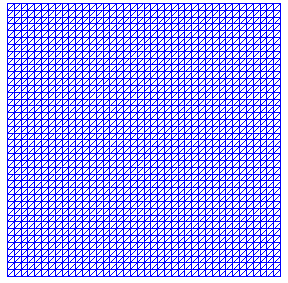
\includegraphics[width=200px]{pics/mesh}
		\caption{Сетка размером $N=40$. Число узлов $1600$.}
		\label{fg:scheme-mesh}
	\end{center}
\end{figure}

\subsection{Эталонное решение}
Для сравнения нормы погрешности вычисляется эталонное ``псевдоточное'' решение ${\bm u}_{ex}^n$, на чисто неявной схеме (\ref{eq:scheme-impl-1}), на сетке размером $N=200$ и $\tau=0.00125$.

\subsection{Норма погрешности}
Вычисление нормы $L_2(\Omega)$ погрешности $\varepsilon^n$ для временного слоя $n$:
$$
\varepsilon^n = \left(\int_{\Omega} ({\bm u}_h^n - {\bm u}_{ex}^n )^2 \, dx\right)^{\frac{1}{2}}.
$$

\subsection{Сравнение}
На рис. (\ref{fg:scheme-L2-1}) - (\ref{fg:scheme-L2-4}) представлены графики сравнения норм погрешности $L_2(\Omega)$  для четырех разных сеток (по горизонтальной оси временные слои, по вертикальной оси норма погрешности). Обозначения схем на рисунках:
\begin{itemize}
\item cn - схема Кранка-Николсона,
\item dr - схема Дугласа-Рекфорда,
\item im - чисто неявная схема,
\item ct - схема расщепления по компонентам,
\item pr - схема Писмена-Рекфорда.
\end{itemize}



Схемы расщепления проигрывают по точности чисто неявной и Кранка-Николсона, при этом  схема Писмена-Рекфорда неустойчива на сетке $N=20$ независимо от $\tau$. При увеличении размера сетки схема Дугласа-Рекфорда заметно приближается к неявной и Кранка-Николсона.

График на рис. (\ref{fg:scheme-time}) показывает, что время вычисления по схемам расщепления быстрее чем по неявной и Кранка-Николсона. Таким образом схема Дугласа-Рекфорда наиболее предпочтительная для решения задач данного типа.

\begin{figure}
	\begin{center}
		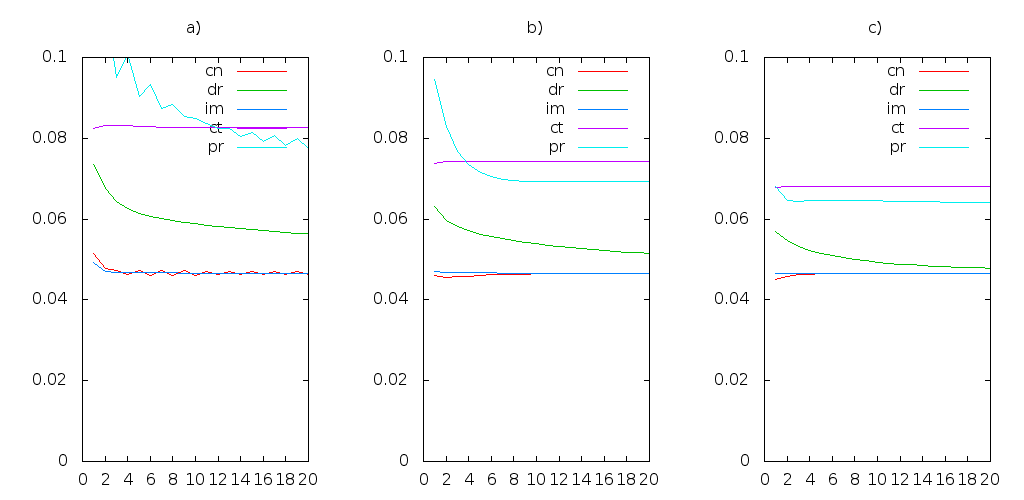
\includegraphics[width=400px]{data160/error_1}
		\caption{Норма погрешности скорости в $L_2$ для $N=20$, a) $\tau=0.01$, b) $\tau=0.005$, c) $\tau=0.0025$.}
		\label{fg:scheme-L2-1}
	\end{center}
\end{figure}

\begin{figure}
	\begin{center}
		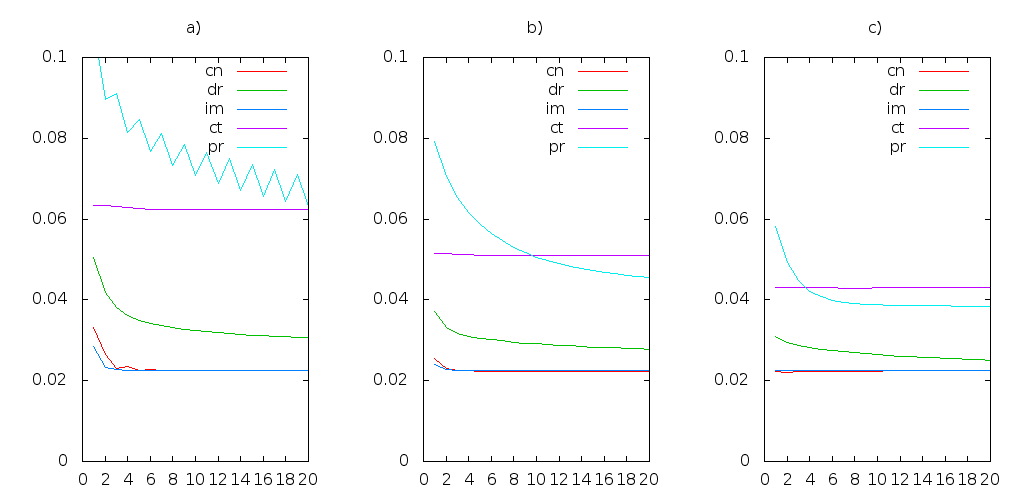
\includegraphics[width=400px]{data160/error_2}
		\caption{Норма погрешности скорости в $L_2$ для $N=40$, a) $\tau=0.01$, b) $\tau=0.005$, c) $\tau=0.0025$.}
		\label{fg:scheme-L2-2}
	\end{center}
\end{figure}

\begin{figure}
	\begin{center}
		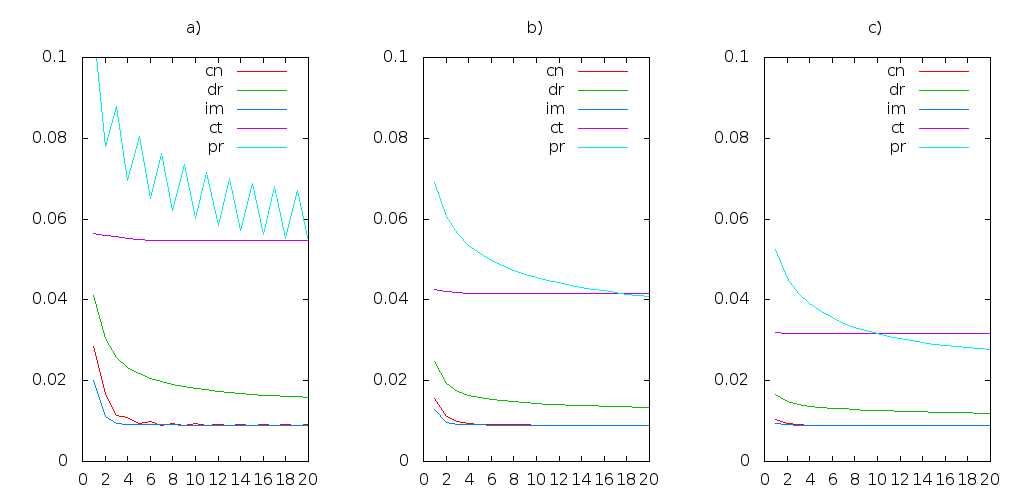
\includegraphics[width=400px]{data160/error_3}
		\caption{Норма погрешности скорости в $L_2$ для $N=80$, a) $\tau=0.01$, b) $\tau=0.005$, c) $\tau=0.0025$.}
		\label{fg:scheme-L2-3}
	\end{center}
\end{figure}

\begin{figure}
	\begin{center}
		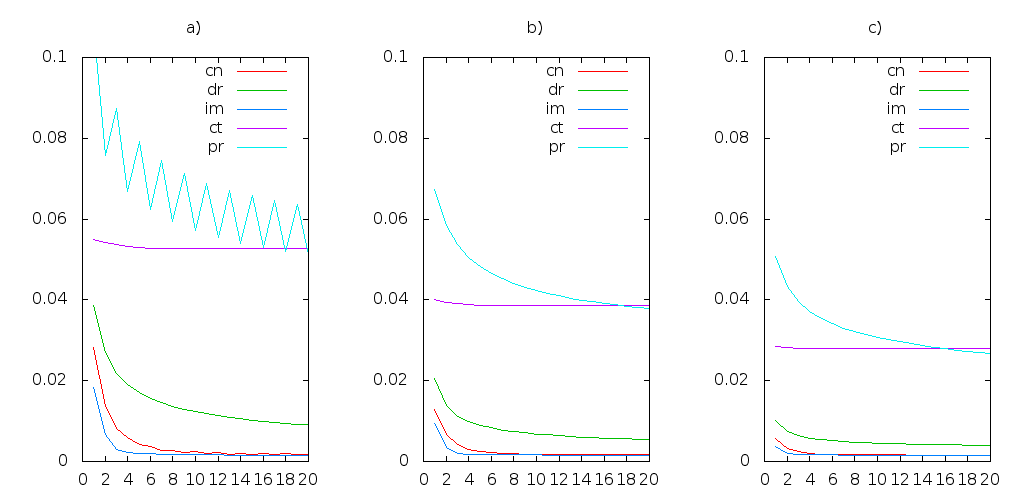
\includegraphics[width=400px]{data160/error_4}
		\caption{Норма погрешности скорости в $L_2$ для $N=160$, a) $\tau=0.01$, b) $\tau=0.005$, c) $\tau=0.0025$.}
		\label{fg:scheme-L2-4}
	\end{center}
\end{figure}

\begin{figure}
	\begin{center}
		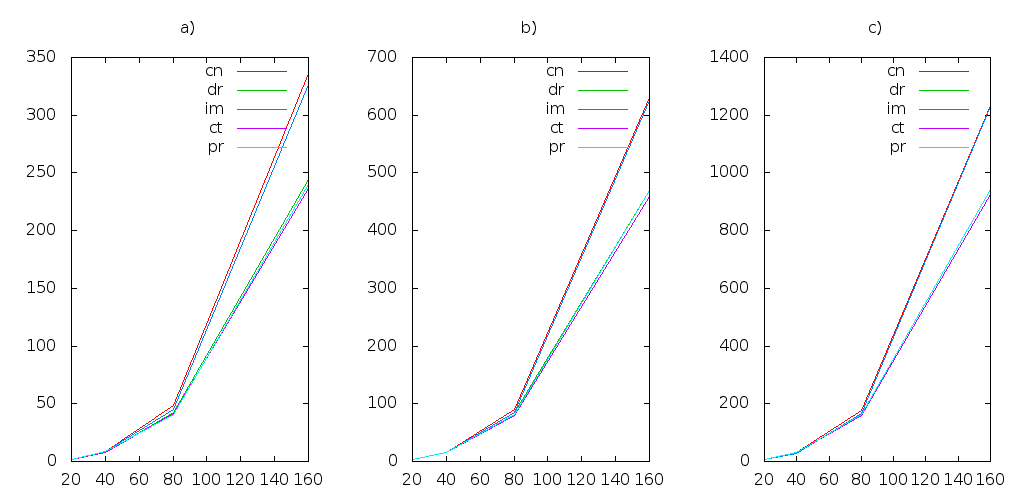
\includegraphics[width=400px]{data160/scheme-time}
		\caption{Время вычисления для a) $\tau=0.01$, b) $\tau=0.005$, c) $\tau=0.0025$.}
		\label{fg:scheme-time}
	\end{center}
\end{figure}

\begin{thebibliography}{9}
\bibitem{vabishchevich-1999} Самарский А.А., Вабищевич П.Н. Аддитивные схемы для задач математической физики. \newblock --- М.: Наука, 1999. 319~с.
\bibitem{fenicsbook-2012} Anders Logg, Kent-Andre Mardal, Garth Wells. Automated Solution of Differential Equations by the Finite Element Method. \newblock --- Berlin: Springer Berlin Heidelberg, 2012. 723~pp.
\bibitem{guzman-2011} J. Guzman, M. Neilan. Conforming and divergence free stokes elements on general triangular meshes. \newblock --- Providence, RI, USA: Scientific Computing Group, Brown University, 2011. 17~pp.


\end{thebibliography}

\end{document}